\chapter{Rituals and Social Traditions}
\paragraph{Rituals.} Many of us believes in rituals but not many think of the
root element of a ritual. We ask ourselves, are we as much humble as
talkative? What would others say about us? We are always afraid of this but
still we never have a good opinion of others.

Now let us think about the rituals. Every ritual happened one time as a result
of people's process and people's arrangement. People means, what is society's
view, what is society's situation and what is society's intention, is important
to understand.

I, you, our relatives, neighbours, and going further, our community and
town-city and country, why do we live together? Why do we accept the rule of
living together? All theories, all beliefs are linked to each other one after
the other. Our each step is decided by a pre-established arrangement.

Discussing this ponderable question in more detail, we find that every deed of
our life has been organized into reasonable or unreasonable by a social system.
Every arrangement has been deemed reasonable by a comprehensive principle. New
arrangement is born from old arrangement. New principle takes fruition from old
one. This is the chain of society. 

For instance, when a child is born, there are some norms decided for his
upbringing. Some system is decided to train him. His marriage is put under some
limits and with regard to his progeny, some responsibilities are decided and
others are denied. These systems, these standards and these responsibilities are
deemed reasonable under some principles of life. A series of these principles
makes a kind of social chain. Each link of this chain fits perfectly with the
other link. This whole chain could be called a social view of life but a main
point is that to create this view of life, some basic points are required.
These, in the absence of a better phrase, could be called the basic elements of
social life. In English, there is a word for this: ``data". A theory can not be
established without sufficient data. But this data is not a thing of logic,
intelligence of humbleness. This data can only be the interaction of facts with
the natural laws. \textbf{These facts and unanimity can not be forever. They
have the limits of time and place. This fact is so clear that it is not required
to put any more arguments in its support.}

Based on your situation and circumstances you think of how will you prosper most
in the future and live within your means is a thing of commonsense. Similarly,
society also plans and programs its future based on the situations and
circumstances. These programs are rituals and the initial thought behind these
rituals are theories.

At some point, some one can say, every ritual might be deemed reasonable based
on some theory, afterall, our ancestors were not foolish to implement them.

Let is see the above point in more detail. Every theory needs some data. The
data available at the time of forming a theory remains forever. The theory
remains valid as long as the data remains valid. If the data changes, then,
based on natural laws and systematic depreciations on theories and opinions, the
nature of these rituals change. As the nature of above mentioned data changes,
the theories behind the data must change and by consequence, the rituals formed
from  the theories must change too, or else the rituals becomes meaningless and
baseless.

\textbf{Inspite of these, if a ritual is followed just because it is coming along from a
long time, the society becomes ritualized and a ritualized society is aimless
society which is like having a roof without walls.}

After this introductory discussion, let us see Thar's main rituals and
traditions.

\begin{table}
\begin{center}
% use packages: array
\begin{tabular}{|lll|lll|}
\hline
(1) & gold: & tuss & (12) & rupees: & visa/khodo\\
(2) & opium: & mung/rati & (13)  &sand  & fistful/handful\\
(3) &mixture to make curd: & chhanto & (14)  &grass  &bundle\\
(4) &butter: & fingers & (15) &kana  &bhakar\\
(5) &snuff: &pinchful & (16) &wood  &log\\
(6) &magat: &chugtho & (17) &melon  & pie\\
(7) &sangri/beans: &fistful & (18) &roti  & piece\\
(8) &buttermilk: &lup & (19) &laddu  &kado\\
(9) &sugar: &mouthful & (20) &ghee  & spoonful\\
(10)&wheat/barley: &gaaro & (21) &sweets  & daboro\\
(11)&dates: &satto & (22) &distance  & vikha\\
\hline
\end{tabular}
\end{center}
\caption{Measurements of different things in common usage}
\label{tbl:measure}
\end{table}

\section{Birth}
Almighty has created a system of birth in this world for the progeny in humans,
animals and plants, etc. For a systemic management of world and society, seers
and saints institutionalized marriage under which woman gets pregnant and as a
result new generation is born leading to progeny of generation. Now let us see
the prevalent rituals related to birth in Maheshwari community.

When a pregnant woman is in her seventh month of pregnancy, the \textbf{hair
washing ritual} is performed.  When the woman is at her in-laws place, the hair
washing was done on \textit{sud} day fifth, seventh, ninth or thirteenth.  At
this time \textbf{khetwar's or kshetrapal's juhar} was done. A brick is washed
and worshipped as a symbol of kshetrapal.  The girl is adorned with
\textit{kumkum chandlo}. \textit{Abil}, \textit{gulaal}, kumkum, 7 cardamoms, 7
cloves were used with a \textit{diya} light and coconut was broken.
\textit{Sawa ser} (750 grams) wheat laduo were made and was worshipped. With
another sawa ser flour, five big \textit{rotas} were made and worshipped with
powdered sugar and ghee. These rotas were eaten by the woman. Along with the
woman, her younger brother-in-law or elder brother-in-law's son used to sit to
eat. The food hence cooked must be consumed before night, and could not be left
for second day. Other things used in worshipping were given to cow. Sweets were
distributed among the relatives. If for some reasons the hair wash ceremony was
not done in seventh month, it is done in ninth month.

In Maheshwari community, since a woman's first delivery is traditionally done
at her parent's place, they are informed in advance. After the hair washing
ceremony, woman's uncle or brother came to pick her up from her in-law's place.
The in-laws used to give a large \textbf{dohti} which was called
\textbf{sadra-ri-reet}. After reaching the parent's place, this dohti was
distributed among relatives, so that people knew the woman is pregnant. After
the ritual of hair washing, the woman has to stay at home. If required to go
out, she had to come home quickly. She was not allowed to go out at late
evening or night at all.

There were no public hospitals for childbirth in Thar. There were no maternity
homes. Experienced mid-wife (who likely used to be the town's barber) assisted in
childbirth. In cases of problems, she knew of home-based solutions but in
serious cases such as if child is inverted, the child or woman would die
because of lack of doctors and hospitals.

Experienced mid-wife and some senior women would predict about the gender of the
child based on the mother's stomach and other characteristics. These
predictions used to be true most of the times. No advanced tools such as
sonography were available in those days.

Birth control devices and abortions were not prevailing in those days. As and
when the child was born, it was accepted as almighty's gift. However, if after
first daughter, second and third daughter were born, dissatisfaction spread
into family. However, daughter is born, so there will be an exchange in
marriage used to be prevailing thought. Sons were more desirable. This was
because, son was the heir of family and was the one who could perform the death
rituals of parents. There are instances of upto eleven daughters born back to
back \textbf{naronar} in the hope of a son out of which 4 died and 7 were married off.

Mid-wife periodically visited to check on the woman. She would also inform of an
approximate date of birth. Childbirth was done at home in a separate room. A
jute bed-cot was used for childbirth. After the childbirth, woman was given
warmth by burning dried cowdung under the bed-cot.

If the newborn is a boy (and that too the first) then the mid-wife would
immediately go th woman's parents to congratulate them and would receive some
prize in addition to regular fees.

In the event of the birth of a boy, people used to beat steel plates with
rolling pin (\textbf{thali vagadvi}) to announce in the neighborhood of the
birth of the boy (if some family had only girls born, people used to taunt:
\textbf{taye ghare thaliye kon vagi ahe}). Woman's in-laws were informed by
telegram or letter. Some elder person from family would go to a holyman
(\textit{maharaj}) and informed the time of birth and asked for child's birth
planetary positions. If there is some troublesome planetary positions, then
rituals were done as per the advise of maharaj. Oil was donated in bronze bowl.

On the occassion of son's birth, relatives used to visit to congratulate the
family. Grandfather offered party (\textit{rihan}) and gave a rupee and coconut
to guests. If no rihan was offered, still coconut and rupee was given.
Celebratory songs were sung at grandfather's place which were called
\textbf{lara}. Such laras were sung for the newborn son. Child's paternal uncle
and aunt also organized singing of lara one day each. Dates and sugar candies
were given to the singing women.

On the sixth day of birth, child's maternal aunt wrote the child's
\textbf{chhatthi}. It was drawn on the wall of mother's room using colored
lines and boxes. Aunt lovingly used to bring clothes and gold ring for the
child while the parents would give some more valuable gift in return. In the
night, a blank paper and pen was kept near child's head so that the god of
destiny could write child's destiny.

After eight to ten days, at an auspicious time, the woman would wash her hair
which was called \textbf{melo matho dhoyo}. Until then, she would not go out of
her room. The child is given a name on this day. The name was given based on
the birth \textit{raashi's} birth-letters. As far as possible name other than
according to raashi were not given. If the name is different than birth raashi,
that name was called \textbf{arak naam}. Maharaj would perform a holy ritual
with holy-fire and would tell the child's name with a blow in its ear. This was
called \textbf{gur funk}. Maharaj was rewarded with appropriate remuneration
\textbf{daxina}.

If the child is born under one of the four lunar constellations
(\textbf{Ashlesha}(Hydrae), \textbf{Mula}(V Scorpionis),
\textbf{Magha}(Regulus) and \textbf{Jyeshtha}(T Scorpionis)) then after 27
days, constellation ritual was performed (\textbf{nakhtar naaita}). At that
time twenty-seven well's water, 27 tree's wood, 27 sea shells, betelnuts,
grapes, drumsticks, copper coins etc. were gathered. Maharaj performed holy
fire ritual. Woman and her husband with the child in lap sit together in the
ritual with heads covered and relatives put color on them. Maharaj would give
name based on the lunar constellation such as Mulchand, Jethanand, Magharam
etc. Twenty-seven children were offered meals.

After the child-birth, woman of the town would visit the mother and child and
would bring sugar nuggets (\textbf{sangan misri}). This visit was called
\textbf{bolan aayi}.

At the time of child's birth, nectar of a green leafy vegetable
(\textbf{maido}, tandalja) and jaggery was given as \textbf{suti} or first
food. Woman was given sweets with spices such as dried ginger and sweets with
mussels cumin (\textbf{churi-ro-wato}). Such sweets were called \textbf{goli}.
At the time of son's name giving ceremony, sweet balls of jaggery were made and
distributed. These sweet balls were called \textbf{baruo}. Other sweets were
also distributed among relatives.

Woman after birth was taken care of by the mid-wife. She would wash her's and
the child's clothes for one month or more. She would give oil-massage to both
and would tie the hands and legs of the child with its body properly which was
called \textbf{tanjyo}. This \textbf{tanjan} continued till six months. For
child's diaper, a square cotton cloth was doubled and folded in a triangle.
This diaper was called \textbf{potro}. When the mid-wife left her duties, she
would get money and mother's old clothes.

After a month, woman would wash her head again. This was called \textbf{achcho
matho dhoyo}. If the child died of some reason, then, the head was washed after
twenty-one days. At this time child and son were fed with water from the
Ganges. After that the woman would take over the household work and would work
in kitchen. Feeding mother would take special care of her own diet. She would
not eat sour, spicy and difficult to digest food so that child remains away
from problems. special care was taken in winters and summers. Child was
exclusively fed with mother's milk. External milk was not given. Even after the
child starts eating food, mother would feed her milk for about one and a half
years. Often mothers would give little opium to child so that it sleeps and
would be convenient for mother to finish chores.

After achcho matho dhoyo woman's husband would come to pick her up from her
parent's place. At this time parents would do a ritual called
\textbf{suat-ri-reet}. Woman would get 10 pairs (\textbf{mudd}) of clothes and
child would get 18-20 pair of clothes and golden and silver ornaments. Child
would get a cradle (\textbf{pingho}) or a small bed-cot (\textbf{michli}).
Mostly the first delivery happened at the parent's place. Second, third and
successive deliveries happened at the in-law's place and parent's would give
two pairs of clothes to mother and son each.

Child's \textbf{khetwar juhar} (kshetrapal's ritual) after birth was done in
the forest. On first Deewali festival of child, its paternal aunt and maternal
grandparents would prepare clay pots and would give sweets and two pairs of
clothes. They would bring this with celebratory drum beating. Similarly, on
first Holi festival, they would bring sweets-clothes. This was called
\textbf{dhundhaniyu}.

If the first son is died and a son is born after that, he was called
\textbf{miyachchiwalo} and his nose was pierced. If a son is born after three
daughters, it was called \textbf{tipokar}. For such children, an additional
sister was named from Maheshwari or Brahmin community so that he has four
sisters. If many children died during childhood, a new born was given clothes
from neighbors and given odd names such as \textit{luno, mirchu, bhugdo} etc.

At home, the father would not talk to or hold the child for 6-8 months as
decorum. Other family members would play with the child lovingly and
enthusiastically.

After three-four years when \textit{bhat} visited, he would record the names
and dates of birth of new born children in the family. If a first son was born
he would get a nice gift (\textbf{sheekh}), sometimes a golden ornament.

\section{Janoi (Sacred Thread)}
Brahmans would certainly weat Janoi in Thar. Earlier, Maheshwaris would also
wear but later on that system decayed. Only before getting married, maharaj
would put the Janoi on which was taken off and put on the basil plant after 2-3
days.

In reality Janoi means a second birth of a child because of which Brahmans are
called \textbf{dvij}. But when Maheshwaris worn Janoi (which was worn over left
shoulder and would go to the right and behind), it was used to tie keys. A man
with Janoi would put the thread over his left ear when he goes to toilet and
would remove when done.

\section{Engagement}
Engagement is called \textbf{veenhaan} in Maheshwari community. These
engagements were usually done at a small age. Engagements could be done in any
bloodline (\textbf{nukh}) other than ones own paternal. (Marwadi Maheshwaris
avoids maternal bloodline in addition to paternal ones). Where there is a close
blood relations, such as uncles and cousins, engagements are not possible.

Owing to a skewed male:female ratio in Maheshwari community, there is often a
scarcity of girls for engagement and thus often boy's engagements were
difficult to do.
The male/female ratio of Tharparker district is shown below: This information
has been taken from the Census of India 1931, Vol. VIII, part 1, Bombay
Presidency. For every thousand people the male and female population was as
follows:

\begin{table}
\begin{center}
% use packages: array
\begin{tabular}{|l|ll|ll|ll|ll|ll|ll|}
\hline
\multirow{2}{*}\textbf{Yr/Reg} & \multicolumn{2}{|c|}{\textbf{1881}} & \multicolumn{2}{|c|}{\textbf{1891}} & \multicolumn{2}{|c|}{\textbf{1901}} & \multicolumn{2}{|c|}{\textbf{1911}} & \multicolumn{2}{|c|}{\textbf{1921}} & \multicolumn{2}{|c|}{\textbf{1931}} \\
%\hline
&M&F&M&F&M&F&M&F&M&F&M&F\\
\hline
Sindh&545.5&454.5&546.2&453.8&548.7&451.3&552.0&448.0&560.2&439.8&561.1&438.9\\
Gujarat&515.0&485.0&514.1&485.9&511.4&488.6&518.6&481.4&522.3&477.7&524.9&475.1\\
\hline
\end{tabular}
\end{center}
\caption{Male/Female ratio in Sindh and Gujarat between 1881 and 1931}
\label{tbl:malefemaleratio}
\end{table}

On taking averages, it is found that in Sindh, the ratio was male:female =
552.3:447.7 and in Gujarat it was male:female = 517.7:482.3. Taking into
account the numbers from six decades, it seems the number of females have been
decreasing in Sindh steadily.

Because of this, the system of \textit{sato} (the system of double in-laws),
might have become popular from early on. If a boy is to be engaged, a girl has
to be offered in marriage. The girl can be boy's sister, cousin, neice or other
relative. When the offered girl was a distant relative, it was a tradition to
return a girl in marriage at a later date.

This system was called \textbf{ningri chhokre re varhe mi dini} which roughly
translates to ``the girl was given in boy's dowry". When hearing of an
engagement, people would ask--who is the girl given as dowry (\textbf{chhokre
re varhe mahi kun buhi ahe})? Sometimes when the boy has went past marriageable
age or the home is weak or if the engagement was not happening because of some
other reasons, more than one girl had to be offered in marriage for boy's
engagement. Sometimes, girl's parents would get "\textbf{pet likhe diyo}" which
means that if the girl has a daughter in future, girl's parents has right over
her hand in marriage and they can use it the way they like.

In addition sometimes ``\textbf{mucharko}" was written which means that if the
girl dies, another girl would be offered and so on.

If sometimes when there was no available girl to offer, boy's father would fix
engagement by paying 5-7 thousand rupees. This was called ``\textbf{bought
bride}". This kind of transaction was not seen in good eye for bride's father.

There are also examples where if one's wife is dead, he would offer her
daughter in marriage for getting married again. 

Because of this system of double in-laws, there were many men who would get old
without getting married and would die single. Such people were called
\textbf{dung} or \textbf{pitar}.

Sometimes, contradictory to the above system, girl's father would find a good
groom and fix the engagement. This was called "\textbf{chhokri sirhai te dini}"
and considered to be a status symbol for boy and his family.

\begin{figure}
\center
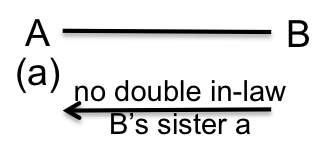
\includegraphics{figures/engagement/straight-sirhai}
\caption{Straight engagement--Sirhai
\label{figure:engage_1}}
\end{figure}

\begin{figure}
\center
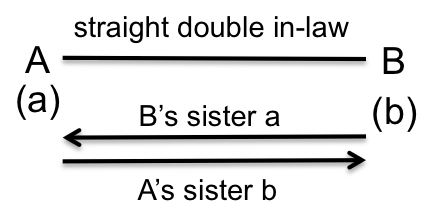
\includegraphics{figures/engagement/straight_opposite_2}
\caption{ Straight engagement Opposite double in-law
\label{figure:engage_2}}
\end{figure}

\begin{figure}
\center
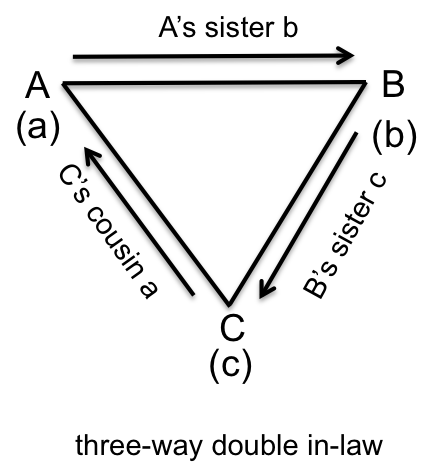
\includegraphics{figures/engagement/triple_3}
\caption{Three-way engagement
\label{figure:engage_3}}
\end{figure}

\begin{figure}
\center
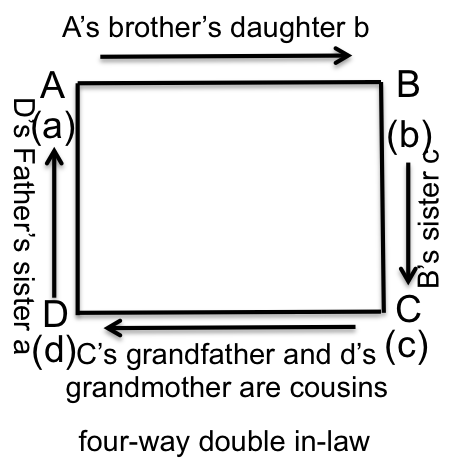
\includegraphics{figures/engagement/four_4}
\caption{Four-way engagement; note: C's grandfather and d's grandmother are cousins
\label{figure:engage_4}}
\end{figure}

\begin{figure}
\center
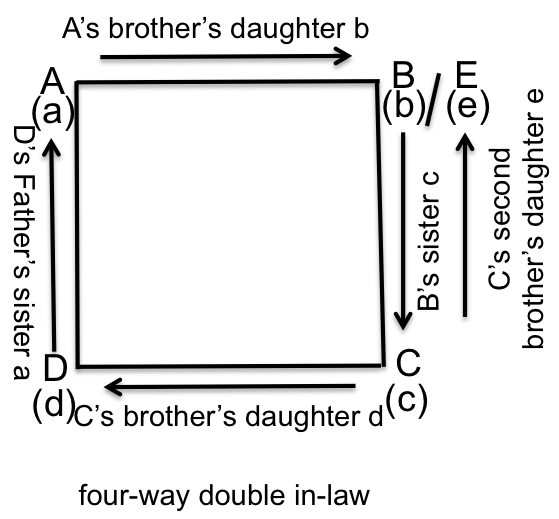
\includegraphics{figures/engagement/four_5}
\caption{Four-way engagement with two girl's offered in marriage; note1: In order to get C engaged, two girls, d and e were offered in marriage; note2: B and E are brothers
\label{figure:engage_5}}
\end{figure}

\begin{figure}
\center
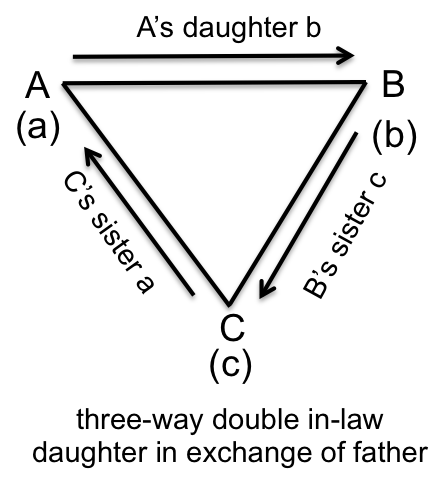
\includegraphics{figures/engagement/triple_6}
\caption{Three-way engagement; Daughter in exchange of father's engagement
\label{figure:engage_6}}
\end{figure}

\begin{figure}
\center
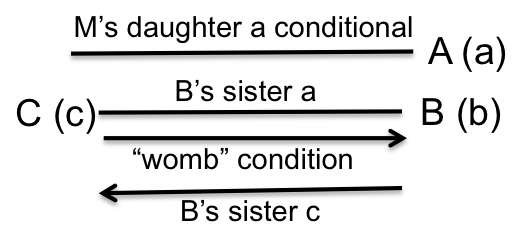
\includegraphics{figures/engagement/womb_7}
\caption{Womb written into marriage; M and N are brothers; a is daughter of M and C is son of N; M's daughter a is married to A and N has got womb written that the future daughter b of A(a) will be offered in exchange of his son C.
\label{figure:engage_7}}
\end{figure}

\begin{figure}
\center
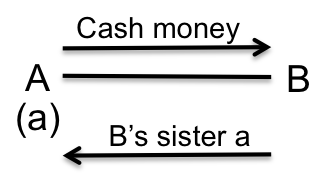
\includegraphics{figures/engagement/cash_8}
\caption{Engagement in exchange of cash money
\label{figure:engage_8}}
\end{figure}

Because of the system of double in-law, straight engagements happened
frequently. Such as a boy and a girl from one home marrying a girl and a boy
from the other. Such cases were possible when there is brother and sister on
both sides. When there are no sisters, distant relative was used as offering.
When there is a spare brother or sister, a third party was brought to use the
system. Sometimes, this happened with a fourth party too. This will be clear
with some diagrams and examples. The examples are taken from real marriages but
names are not given. Instead, alphabetical letters such as A, B, C are used.

In those days, three things were considered when looking for a groom for a
girl: 1) Household--family, 2) Wealth, and 3) Boy. In household--family, the
social image and prosperity--wealth of the family was considered. There wasn't
much cash but it was considered if the family owns land, gold--silver and such
wealth. Further, the boy's profession--employment and his age was considered.

However, since the English education started in Thar and boys started to get
matriculation (around 1918-1919), the education became the most important
aspect to be considered when looking for the groom for a girl. Different
situations demanded different considerations though.

In order to fix the engagement, bride's and groom's parent did not meet with
each other but would use a third-party who is a trusty and known to both the
families. The discussion and conversation would go along for 6-8 months before
the declaration of engagement. If later on there are any disputes between the
two parties, a third party would intervene and addressed the issues. There was
no system of matching bride's and groom's birth planets at the time of
engagement.

When town's elders get together for engagement, they would consider unmarried
boys and girls and set the two- three- or four-ways double in-laws and distant
relatives would communicate the conclusion to everyone involved. In those days
elders were respected and no one could over-ride their decisions. Once the
decision is made verbally, it was considered a fixed decision. Everyone had to
respect the decision.

Engagements were arranged such that the boy and girl could not meet each other.
There was no mutual interview or communication even after the engagement. There
were no photos which could be exchanged.

For the engagement ritual the holymen would be consulted for the right time and
main people of the community would get together at the girl's place. The
engagement was declared there and was registered in a ``\textbf{vahi}" or a
register. The names of both the parties and any double in-laws were registered.
If there is an agreement of a future offering, it was clearly registered so
that there is no dispute later on.

Girl's parents would offer a rupee coin and coconut to boy's parents which they
would accept. People joined from the groom's family would identify people from
the family who are to be given the coin and coconut. Groom's uncle or brother
would announce the names and bride's uncle or brother would bring rupee and
coconuts in a big pan and would go to each of them. The people the rupee and
coconut are offered would take them in lap or in a towel. First coconut was
offered to the paternal family and then to the maternal family. Afterwards the
brothers, cousins, son-in-laws and relatives were offered coconut. If someone
is not present and he is one of the person announced then someone else would
accept on his behalf. The intention of this ritual is to get each parties
introduced to the other parties. After this people would throw color on each
other, have milk and betelnuts and say good bye to each other.

On the other side, the women from the boys side would send milk to girl's
family. Groom's sister-in-law or aunt would carry milk in a colored pot and
walk towards the bride's home. Other ladies from the relative's family would
join them. They would sing along while walking. Bride's family would gleefully
accept the milk. The milk was offered to the people of family and the emply
pots would be returned with small money. Groom's family would bring dresses and
jewelry for the bride and gift it to them. Groom's maternal and paternal uncle
would offer a ``\textbf{mud}" to bride's family. This included a full dress
which happened to be a sari, ghaghro and blouse and in jewellery, golden
head-ring, nose-ring and necklace were offered. In addition, silver anklets
were offered. This system was called \textbf{sakariyo}. After having meal at
bride's place, before leaving, they would offer one sari.

After the declaration of engagement, people from town would go to groom's place
and would congratulate groom's father. They would say ``\textbf{vadhai ahe,
vihan karyo}" meaning ``congratulations on the engagement". On which the father
would reply ``\textbf{thakur vadhaje}" meaning ``god's grace". Rupee coin and
coconut would be offered to people who came to congratulate. Wealthy families
of town or the families who had engagement after a long time would organize a
``\textbf{rihaan}" (party) at the house. Opium, betelnuts and cigerettes were
offered in these parties. Coconut and rupee were also offered. Groom's relative
and family would sing songs which were called \textbf{raaso}. On the second,
third or fourth day, groom's married sisters or aunts may also have
\textbf{raaso} at there place. Women joining in these singings would be offered
seven fresh dates. After the engagement and before the marriage, when there
were festivals such as \textbf{vadi teej}, \textbf{janmashtami},
\textbf{Diwali}, \textbf{Shivratri}, \textbf{Holi} etc., the groom's family
would send sweets such as \textbf{sattu}, \textbf{pedha}, \textbf{gundpaak},
other sweets or dry fruits. Such a sending was called \textbf{bhaado moklyo}.

Engaged boy and girl would never visit their in-law's or in-law's relatives
places. They would not share a vehicle, a seat or would not sit together at a
meal on any social function. Groom would not speak to the in-law's family
members. Groom would never shake hands with his in-law's or any members of
in-law's family. Mother-in-law would never speak to her son-in-law and the
daughter-in-law would never speak to her male in-laws. This kind of decorum was
observed forever from the bride. If a girl is around and her would-be in-laws
appears, the girl would run away.

If a would-be mother-in-law wants to treat her would-be son-in-law, she would
invite her to a neighbor's house. Boy would be accompanied by his 2-4 friends
where the mother-in-law would offer milk to son-in-law and his friends. This
ritual was called ``\textbf{dudh piyaryo}". Everyone would have meal there.
Mother-in-law would offer coconut, handkerchief filled with goodies and dresses
etc. Son-in-law would also offer sweets to children and sister-in-law. 

Son-in-law was addressed with a special prefix or suffix: \textbf{``sahukar or
shah"}. For example if the name is Roopchand, he would be addressed as
Roopchand Shah. This way his respect was maintained.

If the engaged girl dies, the girl's parent would offer another girl or a
relative's girl in marriage so that the other marriages which are linked under
the double in-law system would not break. Sometimes wise people would not break
the marriage and would continue with the other marriages without any amends.

If the groom dies after engagement, the girl would be engaged elsewhere.
Engagements done at a younger age would stay for a long  time, sometimes for
7-8 years. If the girl is too young or there are other obligations and marriage
dates are not fixed for a long time, both parties would understand such
situations and would normally not insist on a fixed date or period for the
wedding. The same understanding prevailed in the case of linked marriages under
the double in-law system. The saying was that \textbf{``vaal vichhaye dinha
ahin to sahe juno paise"} which roughly translates to an expression that if
hair is offered as carpet everything has to be considered.

Sometimes it so happened that a widower would have to be engaged with  the
girl. In the system of double in-law the aim was always groom's marriage and
girl's choices were not given any priorities. Another thing is that if one's
own daughter gets in some trouble after marriage at the in-law's place then the
daughter-in-law was also treated badly to avenge this.

\section{Marriage}
In human life, birth and death are in the hands of almighty. Humans do not have
much control over them. While marriage is organized by the man himself and he
enjoys its bliss. This bliss happens only once in life. (Although man can marry
twice or thrice). Now let us see the old system prevelant in Maheshwari
community:

\paragraph{Deciding the date} After engagement, when bride's and groom's family
think of marriage, they would consult the holymen known to them. The holymen
would suggest 2 to 3 possible dates. Out of these, the date agreeable to both
parties would be decided as marriage date. Some dates required that groom or
bride needed to perform a special ritual which had to be agreeable to both
parties. Mostly people would select clean dates where no such rituals were
required. 

\paragraph{Writing Marriage} Before the date of marriage, on an auspicious day,
bride's family would invite their relatives and 2-3 people from groom's family.
At an auspicious time, everyone would gather at a temple or at bride's home.
Holyman would invite bride's father or brother for a ritual. He would wear a
red turban or an embroidered hat. After the ritual, the holyman would write a
marriage card on a blank paper. He would write the details of bride and groom
and their parent's names, date marriage and planetary positions etc. He would
prepare a \textit{kundali} of the marriage. He would suggest if any additional
rituals are required. The marriage-card would be sprinkled with red kumkum
powder. \textit{Gaudhulik} wedding meaning the time when cows returned in dusk
and dust would fly was considered the best time for wedding or the night time.
Wedding were not organized during the daytime. Holyman would offer yellow rice
and would do a teeka to everyone present at the time of writing marriage. This
meant that the marriage was written in witness of everybody present. In the end
he would collect the yellow rice back from everyone, would add coin, betelnut,
7 dates, turmeric piece and put into the paper and wrap the paper. He would
make a swastik on the paper and would write the bride's name on top. Rupee coin
and coconut would be offered to the people present from the groom's side.
Children would get small money. People would disperse after having smoke and
betelnut. The marriage packet (\textbf{``pado"}) would not be put on floor. It
had to be put on chair or cot. Homes where marriages were written and their
relatives would not go to any funerals until the wedding is over.

\paragraph{Marriage ``sojhna"} Own relatives or neighbor's 4-5 married woman
would perform this ritual. They would put a kumkum swastik on a pan and put a
fistful of salt, rice, moong beans and juwar and would clean and separate them.
The bride would be seated on a cot and they would sing \textbf{``saahevero"}
songs. Afterwards the marriage packet would be tied again. This ritual was
called \textbf{``lagna sohya"}. The participating women would be offered dates.

\paragraph{Sending of Marriage} The products of the above mentioned ``sojhna"
ritual were put in small cloth packets and would be sent to the groom's family
via a gardener. Care would be taken that the marriage packet reaches the
groom's place as soon as possible. Along with the marriage packet, girl's
father would write a letter in which he would write his family's name,
ancestry, salutations to groom's family members and their relatives.
Afterwards, would mention that their daughter's auspicious wedding has been
written and the agreed upon date and would invite the groom's family to come
with a \textbf{``surangi jaan"} or colorful procession to wed his daughter. If
the gardener had to go to another town, they would rent a camel for him. When
the gardener reaches the groom's place, he would be welcomed with water and
salt crystals/nuggets. The marriage packet would be opened and a similar sojhna
ritual would be performed by 4-5 married woman with groom seated on a cot. The
gardener would get 10-20 Rupees as gift and some cloth. He would be offered
meal and groom's family would arrange for his travel back. Groom's marriage has
arrived was soon known to people of the town and they would come to
congratulate groom's family. Everyone was given coin and coconut. Some families
would organize a \textbf{rihan}.

\paragraph{Invitation Card} After the marriage sojhna event, both parties would
write invitations to their relatives. The invitation cards were written by hand
and sprinkled with kumkum powder in those days. If close relatives are in a
different town then the invitation card would be given in person and
hand-to-hand. Sixteen jaggery \textbf{laddu} and 1 syrup \textbf{laddu} were
also given along with the invitation card. Others were sent invitation cards by
post. Care was taken as to see that no relative is forgotten. Close relatives
would take this oppurtunity to steal respect by taking offense and the hosts
would go above and beyond to coax them. Hosts would requestfully insist and say
\textbf{``maahnje otte te chadho"} meaning please come to my home. In extreme
cases bride's father would say, \textbf{``tahje page potiyo rakha to"} which
roughly translates to all my honor is at your feet.

\paragraph{Raw oil} About ten days before the wedding, groom/bride would be
seated on a cot at their home and they would be adorned with oil and songs
would be sung. In order to get the groom up from the cot, his brother or uncle
would say, \textbf{``uthi tana bhalo uth deisa"} meaning, get up, will give you
a nice camel. Bride would also be got up from the cot by her brother or uncle
and she would get money or ring. At this time Bride/Groom's leg would be tied
with \textbf{``laan"} which was a thread with some iron ring, sea-shell and
sealing wax. This was done so that they remain safe of foul play and bad
spirits. Such bride/groom were called oil adorned and would not go out of home
much. Groom would get back massage from a visiting barber everyday. Bride would
also get back massage from a female barber. A \textbf{``devakotho"} would be
painted on the northern wall of home in which Lord Ganesh, Sun-moon,
bride-groom, bed-cushion etc. would be drawn. These were bordered with colorful
boundaries and would look beautiful. Girl's devakotho would have 2-4
riddles/puzzles written over it.

\paragraph{Nanani-Dadani} Bride's maternal and paternal grand parents would
offer one day's meal to all the invited relatives. This was called
``\textbf{nanani-dadani}.

\paragraph{Laapsi} About five days before marriage, groom's family will cook
\textbf{laapsi} and would distribute it to the community. Three people would go
door to door with a large beaker full of laapsi. Two would hold the beaker and
the third would measure 50 tolas (approx. 500 gram) of lapsi and give it to the
family. They would give more if there is any guest in the family at the time.

\paragraph{Vinyakh} Two-three days before the day of wedding (\textbf{paarnet)},
the Vinyakh ritual would take place. Vinyakh means the worship of Lord Ganesh.
Bride/Groom would sit in from on their devakotho on a cot. Songs similar to raw
oil ritual would be sung and all relatives would have meals at the hosts place.
On the right side of the devakotho, a cotton plug dipped in ghee would be
pushed against the wall seven times making seven streams of ghee from top to
bottom. This was called \textbf{maae uthiyarta} meaning remembering the seven
rivers. Groom would wear a big golden necklace.  

\paragraph{Vinaho} Two to four days before the wedding, family's relatives
would start arriving at the family's place. They would bring $1/2$ to 1 kilo of
sweets with them. This sweet was called \textbf{vinaho} and would get
distributed among the guests at the time of meals. Until the wedding sweets
such as \textit{magat} are made, the vinaho was used in meals. This way people
would know who has brought what. At the end of the marriage when sweets were
distributed to departing guests, the vinaho was taken into account.

\paragraph{Mogar} In the home with marriage, the most used sweet was
\textbf{magat}. Rarely was seen a wedding without magat. To prepare magat, men
would be invited from among relatives. A brick furnace would be prepared in the
night. The mogar was made under the supervision of experienced and knowledgable
person. This work was done through labor and community member's cooperation. In
a large deep pan the flour would be roasted. Two persons would stir the flour
with large six-feet long iron spoons. When they are tired, the next two people
would take their place. This way they would all take turns in the activity of
stirring the massive amount of flour. The roasted flour thus made was called
mogar. Adding sugar and ghee to mogar made \textbf{magat}. Everyone present
would eat the magat. Mogar thus made would not spoil for six more months and
magat would be ready in minutes. A detailed recipe for magat is given later.
(Such a process of preparing magat has not been heard of in any other
community).

\paragraph{Siloka} On the night of Vinyakh, and thereafter, there would be
chanting of siloka (god's sloka) at groom's place. 25-30 people would sit
together and one would start chanting slokas. 5-7 people would catch up the
tune enthusiastically. This was called \textbf{tuk jhalai}. People would have
betelnuts, sugar, cigerette, fenel and would leave.

\paragraph{Jaan} Jaan or the marriage procession would go on feet if the
marriage is in the same town. If the marriage is in a different town, they
would hire camels. On the way they would take break and had magat and savoury
fried gram lentils for snack. Magat would be stored in brass pots. Care would
be taken as to who joins the procession. If someone who joins without a
relation then the hosts would say this is \textbf{lakho jaani} meaning a
freebie. When the jaan is about to reach town, the bride family people would go
out to receive jaan. Jaan would arrive one day before wedding. The day the jaan
arrives, they will get camels decorated with adornments and would ride camel
and make camel jump and dance. The groom (\textbf{lado}) would wear soiled
clothes with massage oil and turmuric and a yellow turban so he would be
readily recognized. Lado would distribute money at the time of riding camel.
Elderly women and groom's mother would not join the jaan.

\paragraph{Jaan-ro-dero} The place where the jaan would lodge and board is
called \textbf{jaan-ro-dero}. There, for the convenience of jaan, bride family
would arrange bed, cushions, cots etc. Members of jaan would prepare food
themselves and would eat. Bride's family would send in some snacks. Relatives
of jaan members would send them curd.

\paragraph{Mandhotani} Bride's family would order two festoons from town's
carpenter. It would be colored red. Festoon means three wooden strips joined in
a triangle where in the top two strips are decorated with two sparrows each
shaped wooden pieces and the top angled part is decorated with one sparrow
shaped wooden piece. Five sparrows symbolize five god-godess:
\textbf{``Saraswati samru Sharda, Dhyavu dev Ganesh; paanch dev raksha karo,
Brahma, Vishnu, Mahesh"}. Bride's family would hang to the roof angle, a mud
plate, roti and raw \textit{papad}. Afterwards, the festoon would be tied to
the home's door. After that, they would be accompanied by a holyman and would
go to the jaan-ro-dero. A drummer would beat the drum in front. 5-7 children
would walk with mud plate, perforated wheat flour roti, sugar, cotton thread,
clay pots etc. Men would follow them. House's daughter-in-law would tie a
decorated head band and would carry a colored pot filled with milk. She would
be followed by other woman singing songs. After reaching at the jaan-ro-dero,
people would greet the jaan members and sit together with them. The woman with
milk would be welcomed with salt-water. Groom would do \textbf{``bandai"} to the
milk pot by touching his turban's end cloth to the pot and then touching the
cloth to his face. He would do this 4-5 times. Holyman would tie the festoon to
the door and other things to the hook up the roof. Jaan members would greet
others with cigerette and betelnuts. After a while, they will return back.

\paragraph{Nani Kholo} Groom, Best Man and some friends would sing sloka, stop
frequently on the way and walk to the in-laws place. Best man would be usually
groom's brother-in-law. Best man would carry a bag on his shoulder which had
coconuts and other useful things. In-laws would do the Nani Kholo ritual
meaning would offer a cloth-lungi to the groom and gave coconuts.

\paragraph{Rihan} It was a custom to organize \textbf{rihan} when the
procession came back to groom's town. Groom's father would ask for permission
for this.

\section{Death} 
One's birth can be predicted 7-8 months in advance but death is unpredictable.
Nobody knows when death will happen unless some one inflicts it upon self
(commits suicide), which is a sin religiously and a social and legal crime. If
he gets lucky to live, he becomes unlucky to get punished by law.

Now let us see the prevalant traditions for deaths in the Maheshwari community:
When a person falls ill and has left all hopes of living, at that time a lamp
(with ghee as fuel) is lighted which is called \textbf{jivat divo}. The person
is taken down from the bed. The oldest son would put the person's head on his
lap which was called \text{godo dinho}. Geeta book was read for the dying so
that they can listen to something good. Relatives would declare the donations
they would make in the dying person's name such as grains, milk, ghee, curd,
utensils, grains for birds, animals etc. They would also declare how many
\textit{agiyarash} fast would they observe in the name of the dying. At this
last time family would send ghee and rice to local temple.

Sacred water of river Ganga, basil seeds, and curd is put in the dying person's
mouth. It is said that every form of life gets milk but not curd. Only human
\textit{yoni} gets to taste and enjoy curd. ( It was beleived that the dying
person might not get curd in the next birth. ) A tiny gold grain (\textbf{tus})
was put in an eye. Someone experience would hold the pulse to learn and verify
death.

At the time of last hiccup before last breathe, water was poured over mouth
from a steel pot (\textbf{gagar}). This was called \textbf{paani thyo}. This
was considered very important event. If  this did not happen it was considered
that the dying person's soul went wrong way and the sons of the person were
criticized such as \textbf{moena lap panie kon thyo}. (This tradition was in
place so that the ill person is continuously taken care of and nobody stays
careless. When the breathe stops gets known timely.) At the time of pouring
water everyone would cry loudly so that neighbours would know someone has died.

Dead body's hands and legs would be straightened and the body would be laid
such that the head stays in the North direction. Ear and Nose were plugged with
cotton plugs. Eyes were closed. A brick was placed under their head.

After that in one corner of the room a square was made with cowdung
(\textbf{dhor deita}). The body was washed/bathed, wrapped in a fresh white
cloth and laid down on the square. Forehead was spotted with \textit{Tilaka}.
For the shroud (\textbf{kafan}), a \textbf{nav nali} ( approximately 36 square
feet ). The shroud would be wrapped and sewed on one side and about 1 feet
extra was left open on the other side. This shroud was wrapped on the body with
the open part on the head side. Three small silk cushions were made with cotton
filling.

The funeral processon would start by placing the body on a \textit{nanami} made
of two vertical bamboo sticks and seven horizontal wooden plates tied between
them with jute ropes. Dried grass, dried plant of basil and a small piece of
sandalwood was put on top of nanami. If an unmarried boy has passed away, a
lungi cloth would put as shroud. If a married young man has passed away then
his wife's saree is draped as shroud. Dying married man would be given lungi
from in-laws home called \textbf{ochhado} and if the dying person is a young
married woman, she would be given a pair of clothes (\textit{madd}) from her
in-laws home. If the dying person is an old lady, a necklace made up of basil
wood beads would be put in her neck. Often for the elderly people silken satin
cloth would be used as shroud. The body is tied to the nanami with a sacred
thread and some \textit{gulaal} is sprayed. Dying man's widow would break her
bangles and remove the nose stud. (These were considered the signs of a married
woman.)

Relatives living far away were sent telegrams. However, it took some time for
the telegram to reach and relatives to come so they were not waited for. As
much as possible the funeral procession would start immediately. They would not
let the body stay overnight. However, funerals were never held in night. In the
times of poor communications and transportation, the dying person was given
last rites in the same town where he died.

Before the procession, the relatives of the dead would circumnavigate the
nanami and pray for the departed soul's piece. Barbers were called to home to
shave off hair, beard, moustache etc of the brothers and sons of the dead. If
someone does not want to clean shave head then the sideburns were shaved and
was said to have \textbf{sirbadra dinha}. This was an indication that someone
in the family has died. Relatives would also put coconuts near the body which
was taken with the funeral.

Townsman would reach the cremation ground with a \textbf{kumbhat} wood load on
his camel. This wood would weigh about 100-140 Kilogram. Family's daughters in
law would clean the floor from the place the body is put to the street outside
the home. They would use their saree to dust the floor. This was called
\textbf{vehdo boharyo}.

To give shoulder to the nanami, first great grandson then grandson, son,
brother, daughter's son etc would be the order. If the dying person has great
grandson, it was said he has a golden stairs to heaven meaning he has lived a
happy and fulfilling life. Nanami was lifted such that head remains on the
front. Two people in the front and two in the back, when they lift the nanami,
everyone would cry loudly. Nanami would leave from the main door of home. There
have been instances where daughter's marriage ceremony is about to take place
and father dies. In such cases nanami is taken out from the back of the house,
in some cases after breaking the court wall of house. Dying person's elder
relatives such as father, uncle, elder brother etc. would not join the
procession to crematorial grounds. Husband would also not join the cremation
procession of his wife. Women would also not go. However, women would go to
some distance in elderly person's procession chanting religious songs
(\textbf{bgajans}) and return back. At the time of procession to crematorial
grounds, household and neighbourhood women would cry which is called
\textbf{munhda odhti}. 

During procession, three balls of wheat were made. First was given to dog/cow
at the time of beginning the procession, second at the time of reaching
(\textbf{vesahi taane}) and third at the time of cremation.

If death has occured during some special time of calendar year such as
\textit{panchak} five such wheat floor balls were taken. It was said that a
dying person during the time of panchak would cause death of five more people
from the community. To avoid this, five wheat balls were made. Other people
would take some grains tied in towels and would give those grains to birds at
the crematorial grounds. They would wrap the towel in their necks. One person
would chant \textit{``raam naam satya hai"} from behind the procession which was
repeated in chorus by others. They would chant this all the way. Dying person's
relatives would change shoulders among themselves. Relatives would throw sugar
\textit{patashas} and coins during the procession.

A little before the crematorial grounds, at a predecided spot, after sprinkling
some water on the ground, the nanami would be brought down to the ground. The
end of the cloth shroud would be torn and tied to a tree. The nanami would then
be turned. Now the original people who lifted the nanami in the beginning of the
procession would come back to the nanami and it would enter the crematorial
grounds.

At the crematorial ground, after pouring some water and grains, nanami was put
on floor. A place where there is no recent cremation, wood is arranged after
putting a coin and some water sprinkles. Some dried grass was put on top. Then,
the body was put on top with head to the North direction. Ghee was applied on
body's hands, legs, forehead etc. Then after putting more wood on top the pyre
was completed. Some coconuts were also put in between.

Initially, all four people who gave shoulders or the eldest son would
circumnavigate the pyre and would put fire to the right toe of the body.
Everybody would sit at a distance. 2-3 experienced people would inspect the
pyre frequently. They would turn the wood or if required added more ghee and
wood. Special care was taken so as no part of the body is left unburnt. Such
parts were brain and women's waist. After the pyre is burnt fully, people would
return after bowing to the pyre.

These cremators would go straight to the village well where their children
would be waiting for them with fresh clothes. They would take bath in the same
clothes as they are wearing and then change into fresh clothes. If one has to
bath at home then they would go to the dead person's home. One person who has
already been taken bath would bring some water from inside the house and put
some on each of the cremators head. After this, other than family members, all
would disperse. As cremators come back near home, they would cry. Cremators
from the family would bath at home with clothes on and then would change into
fresh clothes. Died person's son would go to his mother and console her. Roti
was offered to cow and dog and grains to birds.

Meanwhile meals get cooked at home or at the neighbour's. If the died person is
young then pearl millet (\textbf{bajra}) roti and rabdi/moong dal was cooked
and of the died person is elderly then wheat \textit{tikli} (a type of roti)
and dal was cooked.

Everyone would have meals together so that the close family members would also
eat something and would not feel too sad. Until the 11th day at home everybody
would observe \textbf{sutak}, meaning nobody would go to temple and nobody
would do any worshipping at home. 

In third day, \textbf{teiyo} was observed. At this time, relatives in the town
were asked to wash their heads. Everyone would get together and with a
\textit{maharaj}, 2-3 people would go to the crematorium. Others would go to
the well. A water container and some milk would be sent in advance to the
crematorium with which the pyre would be cooled down. This was called
\textbf{chita tharta}. Bones were collected from the pyre and take them to the
well. There, near a peepal (sacred fig) tree the late person would be given
last rites. First the son and then brother etc. would take some water, milk and
leaf and pour some water from hand (108 times) on the ossified bone put on top
of a wheat flour ball. Those who have worn janoi (sacred thread) would do the
same with the thread held between thumb and small finger. After this, they
would put fuller's earth (\textbf{mait, multani mati}) in head and wash it with
water and return home. The ossified bones would be wrapped in a silk piece of
cloth. Alongside \textit{panchratna}(five metals-gold, silver, iron, copper and
brass) and honey would be put and this all would be wrapped in deer skin. Some
fuller's earth would be applied on top and then this would put in a box. This
box was not put on floor but in cupboard or some shelf.

If no lamp has lit then after washing head on teiya, they would lit a ghee
lamp. Died person's son or grandson would take care of the lamp which was
called \textbf{dive betho}. He was given everything to eat that he wished for
such as sweets etc. It was beleived that these things will reach the died
person. The lamp was kept alight continuously. 

This boy would offer rites everyday with water, milk, leaf and wheat flour ball
with 108 times water pouring using both palms near the peepal tree. Alongside,
another person would carry water in a bucket and a metal pot. After the day of
death, each day the flour balls would be increased which became 11 at the
eleventh day. After the rites, the ball was given to cow which was called the
\textbf{bahar-ri-kriya} ritual.

On the day of teiya, died person's in-laws would offer rice and ghee which was
called \textbf{ras dino}. On that day other relatives would wear turbans. Close
relatives would tie some cloth on head until 11th day. Sons and brothers would
not wear shirt. On that day a holy person or priest (\textbf{maharaj}) would
start reading \textbf{garudpuran} which was listened by the women of the
family. 

If the died person is elderly, then the in-laws of their sons would come with
color and would offer a rupee coin and coconut.

On the day of teiya distant relatives were written letters which included the
news of the death and the date of death and dates of 11th and 12th day. Right
corner of the postcard was torn off so that the receivers would know the letter
is about death news.

In the evening of teiya, in a lid of earthen pot, sweets, food and opium etc.
(things liked by the departed soul) with an iron tong and water would be taken
to crematorium. In a street by the crematorium, the lid would be put on floor
and the water would be poured around. The iron tong was taken along so as to
avoid some evil spirit talking the food away.

Men would sit at the home of the departed sould for 12 days. They would spread
sheets etc. (\textbf{tapad vichhaye}) and sit on it. People from town or other
towns would arrive to console the family. They were offered cigarettes,
betelnuts and opium. Women would fold double the end of their saree and put on
their head so that they can put the saree over their face and cry
(\textbf{ochhingar}) when they see some relative coming to console them. This
type of doubled folded saree would also serve as a sign that the woman has
someone passed away in the family.

Household's oldest daughter-in-law, married daughter, or maternal and paternal
aunt's were the main women sitting in mourning. Younger women would do chores.
When some other women come to console, they would also join in mourning.
Depending on the departed soul's age, situation, they would sing mourning songs
(dirges). Visiting women would join in mourning for some time then would pull
the saree over the head of the host woman and would console her to calm down
(\textbf{maat karaiti}). Women of house and visiting women would not wear
\textit{bindi} on forehead. This ritual would continue for months.

Relatives living in other towns, as and when they come to know of the
departure, they would inform others in the town about the death and would say
\textbf{paani ro kahije ta} which would mean that others will come to their
home to console. The relatives would do the water rite 108 times as mentioned
above. They would also sprinkle water over the gathered people and then
disperse. Women would mourn similar to women of the departed person's household
by double folding saree and putting it over their face.

After teiya, the departed's relatives would eat at their house. The relatives
would sleep on floor on a sheet without matress (\textbf{ukhrade}).

On the midnight of the tenth day the lamp would be taken by the boy to a place
with crossroads \textbf{vathan} or \textbf{chovate}. He would dig a small pit
and store the lamp there. He would sprinkle some water. Person taking this lamp
would not speak and would not look back.

Closer relatives from other towns would come on 11th day to visit called
\textbf{kaanehaar} while distant relatives would come on 12th day. If the
visitor is a close relative, he would put a cloth on his head as he comes close
to home and would start crying aloud while coming to the home with wailing
sounds like \textit{ohh my uncle} (\textbf{he mahnja kaka}) or brother or any
other name depending on the relation. This way it would be known who is the
person. Visiting women relatives would also cry like this. Visitor would sit
near the door where someone from house would come and give water. After
drinking water, wherever the mourning is happening, he would sit on the corner
for sometime and then would get up and go to the main person and would console
him by hugging. This is called \textbf{sampharto}. Or, he would shake hand and
say kind words, eg. \textit{ram-ram} and ask about wellness. Similarly, he
would say \textit{ram-ram} to other people around and would sit down.

Visiting woman on \textbf{kaanehaar} would also \textbf{sampharti} to host
women, elderly men etc. depending upon relationship. Such mourning would go on
continuously.

Priest or holyman would assist the son of the departed in 11th day rituals.
They would sit near the sacred firepit, would chant mantras and do rituals so
that the departed soul could rest in piece. They would add grains-sesame-ghee
to the sacred firepit. They would add sutak to the fire. This was called
\textbf{ote-ri-kriya}. In memory of the departed, who would do what kind of
donations and fasts, that would also be declared. In the 11th day meal, they
would cook sugar \textit{halwa} and close relatives would eat together. After
things get burnt in the sacred firepit, the priest or holyman would also have
meals.

Priest would help tie turban (\textbf{potia ra var deraita}). For this
ceremony, people from community would be invited. Priest would do a tilak on
forehead and would give basil leaves to them. This ceremony would mark end of
mourning. However, in reality, some kind of mourning would continue for 8-12
months.

In-laws would put on shirts over the mourning hosts. Father-in-law would offer
money to their son-in-law. Visiting daughter and her \textbf{vejada} (children)
would get clothes and sweets. If the departed soul is a parent of a married
woman, she would also get some gold jewelry. Visiting people would give money
to departed's widow which was called \textbf{thigdi ra paisa}.

If possible, the departed's son, nephew or brother would carry the ossified
bones to Pushkar or Haridwar. They would put the ossified bones in bag/suitcase
and hold a wooden stick with them. Before leaving they would call the departed
by relation or name eg. father/mother/uncle come with me (\textbf {mi bheda
halo}). He would not look back and would not speak. On the way when he would
dine, sit or sleep, he would ask the departed's soul to sit, sleep, eat etc.
After reaching, he would do the appropriate ritual with the help of local
holyman, offer meals to the holymen and appropriate donation for the rituals.
This ritual was called \textbf{taravto} meaning letting the departed soul's
ossified bones be merge into the holy waters. He would also register his name
on the registries maintained by the local holymen. After this ritual, he would
let his head shave there. He would return after finishing everything.

If no one is able to go to Haridwar or Pushkar for this ritual, the box with
ossified bones would be sent by post or parcel to the holyman and they would
themselves do the rituals. The donation for holyman would be sent via
moneyorder. Such holyman would visit Thar's villages once every 4-5 years and
would obtain some money as donation.

On the 12th day, the departed's son would go to \textit{dhura} (a division of
community), would wear towel around neck and would request \textbf{assanje
vadil ri osser ri mokal dyo} meaning grant permission to organize a community
feast in memory of the departed soul. For this there was a special saying as
\textbf{muth ghughariya ri karan do}. Depending on the past deeds by the family
on other similar occassions, the dhura would accordingly grant permission.

A community rihan is organized on 12th day where opium was used. After that, in
sweets \textit{dahithara} (a sweet made up of curd)/\textit{jalebi} (a sweet
made up of fermented flour, oil/ghee and syrup)/\textit{bundi} (a sweet made up
of chick peas floor, ghee and sugar) (in increasing order) would be cooked
depending on one's status and position. If some likes to do \textbf{panch
pakwan} they would cook five sweets as \textit{bundi}, \textit{jalebi},
\textit{dohti}(a sweet made up of flour, ghee, sugar), \textit{mesu},
\textit{mohanthal}(a sweet made up of chick peas flour, milk, sugar, ghee).
Brahmins were said to have done Brahmbhoj. Each Brahmin with sacred thread
would be offered a donation of a rupee or more.

Arriving Brahmin would have meal for himself and would take a fixed amount of
sweet per family member at the time of leaving. This is called \textbf{biro}.

Dhura's guests arriving for feast would bring their own utensils, cold water,
poppadams, pickles etc. Feast would happen in the street where everyone would
eat together.

Such community feast was called \textbf{mahajan} and when done by Brahmins, it
was called \textbf{maastaan}. If someone organizes this kind of feast in memory
of their departed elders then it was said that one has done
\textbf{mahajan-maastaan} and this would get registered in community holyman's
registers.

Maheshwaris would spend a significant amount of money in such \textbf{ossers}.
For poor people, this would mean that all their savings would get washed off
and they might have to take loans to organize such events.

In memory of the departed, priest would read \textit{Garud Puran} from teiya
till 13th day. It would end on 13th day.

People who have visited in kaanehaar would also offer some donations to the
priest reading the Garud Puran which was noted in a notebook(\textbf{bandi}).
Additionally, family would give cot, duvets, beddings, cushions, mattress,
light, cow etc in donation. Instead of real cow, a symbolic token of small
silver cow would be given which was said to help the departed reach heaven. It
was said that the departed would hold the tail of this cow and swim across the
Vaiterni river and would reach heaven.

After the 12th day, almost everyone would disperse, only close relatives would
stay. On 17th or 18th day \textbf{Maasi chhant} (monthly ritual) would be done
when the priest would be offered meal and a donation. After this everyone would
leave. Six monthly and annual ritual would be respectively done on 5th and 11th
month during the waning (\textbf{vad}) part of the lunar calendar. Family
members would be invited for six monthly and annual rituals by writing letters.
Brahmin would do sacred fire-pit ritual and would obtain a donation.

After the departed's death date, one \textbf{shraaddhs paksh} would be left and
in the next \textbf{shraddh paksh}, their first \textbf{shraddh} would be
observed. At this time all the relatives would be informed by postal letters.
Sweets such as \textbf{kheer} (a kind of rice pudding) and
\textbf{muthia-ra-laddu} (a sweet made up of flour and ghee) would be made.
Alongside wheat floor \textbf{tikli} (a kind of roti) and
\textbf{chibhde-karing-guvar fali ro saag} (mixed melons vegetables) would be
cooked. More than one brahmins would be invited for meals. After that, on each
of the Shraaddhs, only family members, a brahmin and daughters would be invited
for meals.

Widow would not step out of house until after the first Shraaddh of the
departed which was called \textbf{khuno paadyo}. Such a thing would sometimes
happen for two years (if a person is dies just after the Shraaddh paksh, his
Shraaddh would be observed after two years). After first Shraaddh, woman's
parents would take her to their home and would offer her a new pair of clothes.
This was called \textbf{khuno chhadayo}(she can step out the door now). 

\paragraph{Vaikunthi.} If the departed is a leading person in the community and
of upper status then their children would celebrate a vaikunthi for them. For
this, the corpse would be bathed and arranged such that it is sitting upright
with straight neck. 

A wooden chariot would be made with three sides open and the back side closed.
The departed would be seated straight on this chariot. The chariot would be
decorated and there will be four handles around it which would be lifted by
four turbanated people. Red color powder (gulaal) would be sprinkled all over
during the procession. Also, money and sugar candies (\textbf{patasha}) would
be distributed along way.

Temples on the way or all temples in the town were visited and the procession
would stop for a short while. The pyre would be set with the body straight in
seated position and wood etc. would be arranged around it. Before doing
Vakunthi, a permission was sought from the community and the community will
consider all the relavant factors and past of the family before making
appropriate decision.

The meals would include panch-pakwan. Mahajan-Maastaan would be offered meal.
Brahmins would get good donations.

After the formation of Pakistan, in Mithim Ranchhod-das Bekhatmal Dhirani and
his brothers celebrated Vaikunthi of their father, Mr. Bekhatmal. This
Vaikunthi was celebrated on 24/03/1982 which was probably the last in Thar.
Then, the departed's sons offered meals to the whole town of Mithi (including
community and non-community people such as muslims). In other towns of Thar
where Maheshwaris lived, they sent special people to cook sweets the same day
and distribute to Maheshwari households.

\paragraph{Infant or Child Death.} If an infant or a child is died because of
diseases such as Pox then they would be buried instead of cremation. After
wrapping them in appropriate shroud, digging a pit and the child would be
rested in there. Some salt would be sprinkled over the body so that it gets
dissolved in soil faster. Some thorns would be spread on top and then the pit
would be covered with soil. Thorns were put so that some animal may not dig the
pit and disturb the body.

\textbf{Note:} Elderly person, if passes away, it was called \textbf{``Ram
karyo"} and if a child passes, it was called \textbf{``pachho thayo"} meaning
``returned back".

\subsection{Dirges}
Dirges are called ``par" in Dhati. Women sing them while mourning behind a person who passes away. Such dirges were sung about the person's life, their age, the family they left behind etc. Even after trying no woman (or man) was ready to sing these dirges, so they were not recorded here.

Widowed woman would normally sing dirges behind their husbands like so:\\
\textbf{hey hu to muthi} (became widow)\\
\textbf{hey mahnja bachiya na role gayo} (left my children alone)\\
etc.

